\documentclass[border=0.2cm]{standalone}
\usepackage{tikz}
\usetikzlibrary{angles,quotes}


\begin{document}
\thispagestyle{empty}
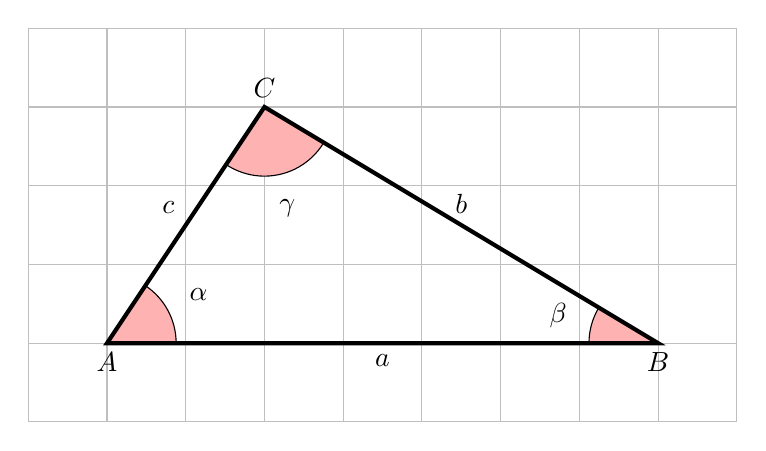
\begin{tikzpicture}

\draw[step=1,gray!50] (-1,-1) grid (8,4);


% Coordenadas dos vértices
\coordinate (A) at (0,0);
\coordinate (B) at (7,0);
\coordinate (C) at (2,3);



% Etiquetas dos vértices
\node[below] at (A) {$A$};
\node[below] at (B) {$B$};
\node[above] at (C) {$C$};

%\pic [draw, "$\alpha$", angle eccentricity=1.5] {angle = A--B--C};

%\pic [draw, "$\alpha$", angle radius=15pt, angle eccentricity=1.5] {angle = B--A--C};
%\pic [draw, "$\alpha$", angle radius=15pt, angle eccentricity=1.5] {angle = A--C--B};
%\pic [draw, "$\alpha$", angle radius=15pt, angle eccentricity=1.5] {angle = B--C--A};


% Desenhar os ângulos nos vértices
\pic [draw, "$\beta$",  fill=red!30, angle radius=25pt, angle eccentricity=1.5] {angle = C--B--A};
\pic [draw, "$\alpha$", fill=red!30, angle radius=25pt, angle eccentricity=1.5] {angle = B--A--C};
\pic [draw, "$\gamma$", fill=red!30, angle radius=25pt, angle eccentricity=1.5] {angle = A--C--B};

% Desenhar os lados do triângulo
%\draw (A) -- (B) -- (C) -- cycle;
\draw[line width=1.5pt] (A) -- node[below] {$a$} (B) -- node[above] {$b$} (C) -- node[above left] {$c$} cycle;

\end{tikzpicture}

\end{document}
